\documentclass[10pt]{article}
\usepackage[utf8]{inputenc}
\usepackage[T1]{fontenc}
\usepackage[polish]{babel}
\usepackage{times}
\usepackage[a4paper, total={6in, 9in}]{geometry}
\usepackage{graphicx}
\usepackage{pythonhighlight}
\usepackage{subfig}
\usepackage{float}
\graphicspath{ {.} }


\title{
\rule{\linewidth}{3pt}
Klasyfikator ruchów czujnika IMU na podstawie rekurencyjnej sieci neuronowej
\rule{\linewidth}{1pt}
}
\author{
  \textbf{Mateusz Woźniak}\\
  \texttt{wozniakmat@student.agh.edu.pl}
  \and
  \textbf{Maciej Pawłowski}\\
  \texttt{maciekp@student.agh.edu.pl}
}
\date{}

\begin{document}

\maketitle

\section{Abstrakt}

Przedmiotem tego artykułu jest omówienie realizacji zadania klasyfikacji ruchów z urządzenia IMU (Inertial Measurement Unit). Czujnik IMU określa przyśpieszenia postępowe i kątowe używając żyroskopu, akcelerometru i magnetometru. 
IMU jest powszechnie stosowane w lotnictwie, robotyce, wirtualnej rzeczywistości i medycynie. W lotnictwie umożliwia precyzyjne sterowanie statkami powietrznymi, a w robotyce wspomaga autonomiczne poruszanie się robotów. Jednym z zastosowań klasyfikatora ruchów może być detekcja przeciągnięcia samolotu. Z kolei w motoryzacji, IMU znajduje użycie w systemach kontroli stabilności pojazdów oraz w zaawansowanych systemach wspomagania kierowcy, które poprawiają bezpieczeństwo. My chcemy zaproponować realizację klasyfikatora 5 z góry ustalonych ruchów używając rekurencyjną sieć neuronowej. 

\section{Zbiór danych}
Dane zostały zebrane z urządzenia Samsung Galaxy S10e 2019. Każdy ruch został zebrany ręcznie a seria danych z czujników była zapisywana do pliku $csv$ o ilości wierszy takiej jak ilość kroków czasowych. Interwał samplowania pomiaru z czujnika ustaliliśmy na $50ms$. To znaczy, że w ciągu każdej sekundy trwania ruchu następowało 20 odczytów.

Ruchy były wykonywane przy włączonej aplikacji mobilnej napisanej w Kotlinie (rys. 2).

\begin{figure}[h]
\label{fig:screenshot}
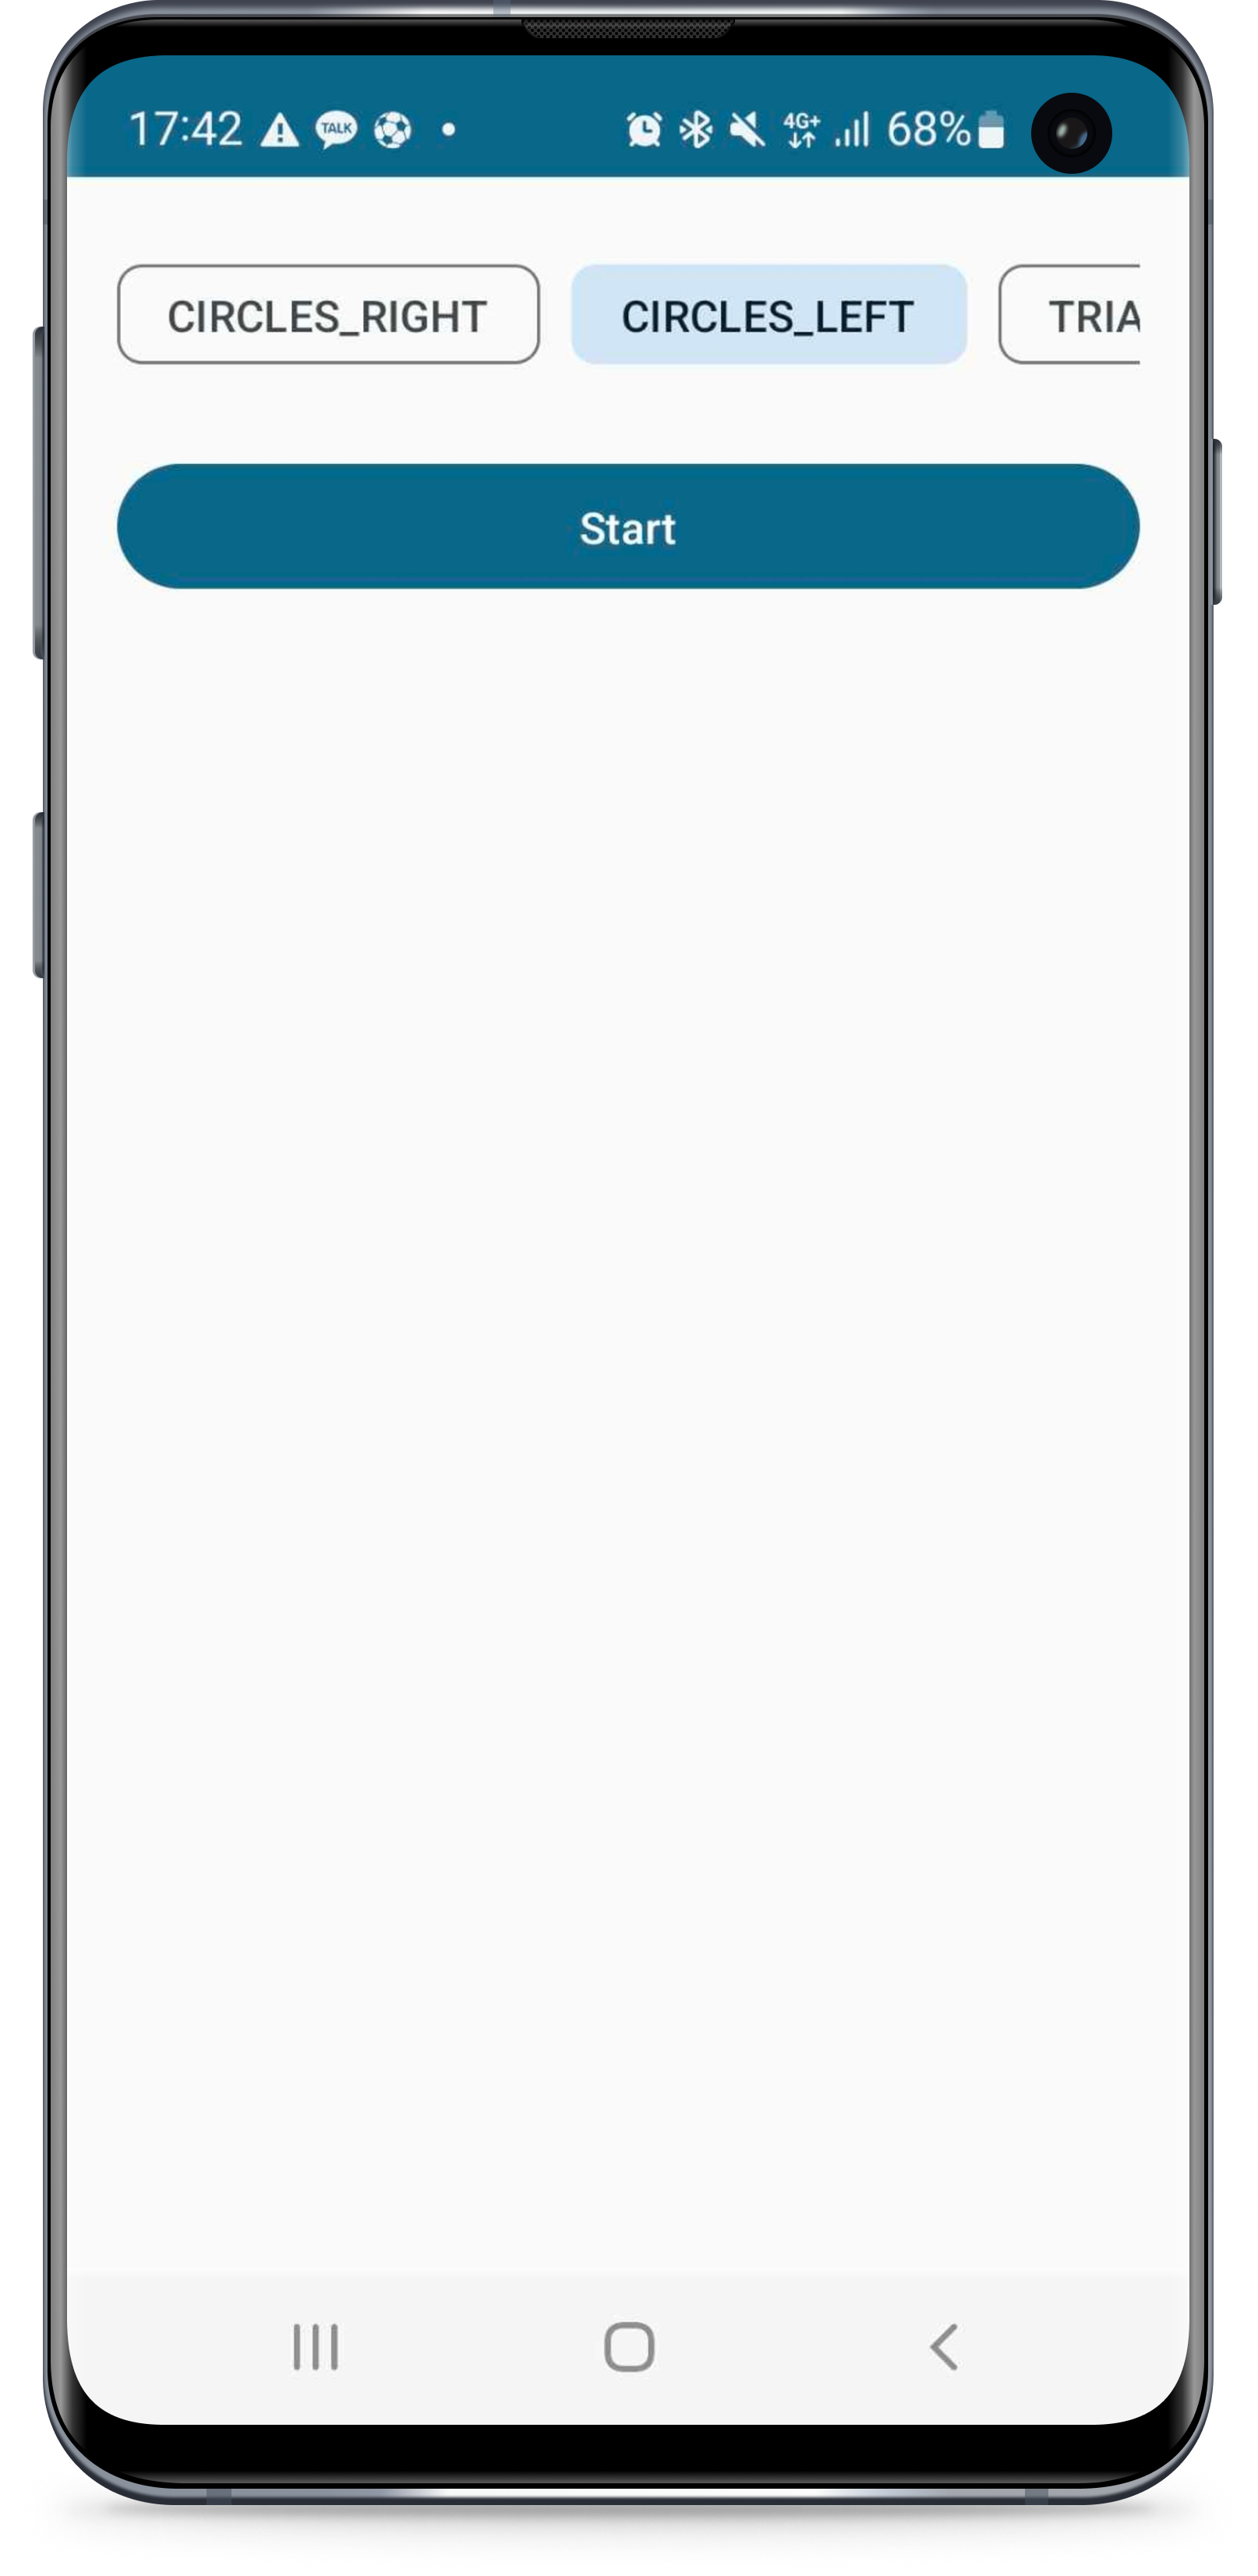
\includegraphics[width=5cm]{s1.png}
\centering
\caption{Aplikacja mobilna do zbierania danych z czujnika IMU}
\end{figure}

Dane były wysyłane na zdalny serwer na którym był uruchomiony mikroserwis HTTP napisany w Go. Mikroserwis zbierał dane i zapisywał je na dysk. Dzięki temu zbieranie danych odbywało się sprawnie, a mikroserwis dawał nam informacje o ilości ruchów dla każdej z klas.

Przykładowy plik $csv$ (oraz jego wizualizacja na rys. 1):
\begin{verbatim}  
gyro_x;gyro_y;gyro_z;magnetometer_x;...
-0.062384613;-0.15294538;-0.32650748;-43.62;...
-0.87361366;0.41210496;-0.49510628;-43.5;...
-1.7758616;0.20685424;-1.4266758;-43.92;...
-1.8662697;-0.46876273;-1.4040737;-44.399998;...
-0.7575493;-0.8077929;-1.488984;-44.28;...
0.06895141;-1.5170075;-2.1273382;-46.14;...
\end{verbatim}


\begin{figure}[H]
  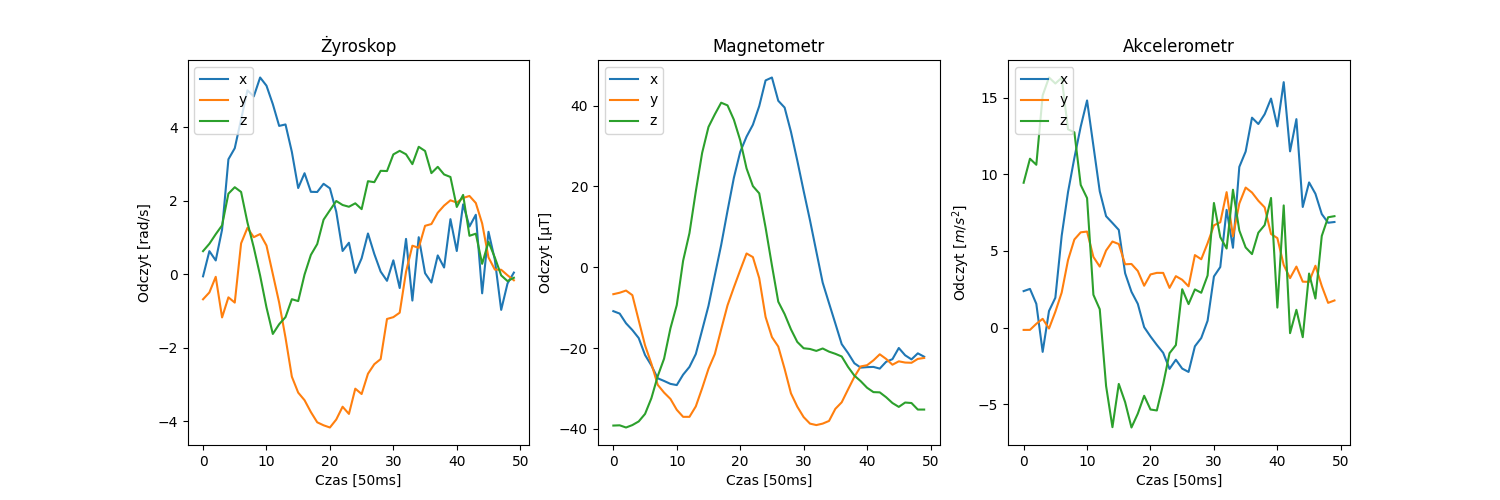
\includegraphics[width=16cm]{sample.png}
  \centering
  \caption{Przykładowy odczyt ruchu dla klasy CIRCLES\_RIGHT}
\end{figure}

\pagebreak

Zebraliśmy dane dla następujących klas:

\begin{center}
\begin{tabular}{ |c|c|c| } 
  \hline
  Klasa & Opis ruchu & Ilość sampli \\ 
  \hline
  SQUARE & Ruch imitujący rysowanie kwadratu & 203 \\ 
  \hline
  TRIANGLE & Ruch imitujący rysowanie trójkąta & 179 \\ 
  \hline
  CIRCLES\_LEFT & Rysowanie okręgu przeciwnie z ruchem wskazówek zegara & 193 \\
  \hline
  CIRCLES\_RIGHT & Rysowanie okręgu zgodnie z ruchem wskazówek zegara & 191 \\
  \hline
  FORWARD\_BACK & Ruch "od siebie - do siebie" & 187 \\
  \hline
\end{tabular}
\end{center}

Dane zostały załadowane do tensora o kszałcie $(B, T, C)$, gdzie
\begin{itemize}
\item $B$ - wsad (32)
\item $T$ - oś czasu
\item $C$ - cechy (9)
\end{itemize}  

W przypadku, gdy sample były różnej długości, tensor został dopełniony zerami, by $T$ było równe 100. Dzięki temu tensor stawał się jednorodny [4]. 

\section{Model}

Ze względu na to, że zadanie klasyfikacji ruchów ma być niezależne od czasu, tzn. że ruch może zawierać dowolną ilość sampli zdecydowaliśmy się użyć rekurencyjnej sieci neuronowej z komórką LSTM.
Long Short-Term Memory (LSTM) to rodzaj architektury sieci neuronowej rekurencyjnej (RNN), zaprojektowanej w celu przezwyciężenia ograniczeń tradycyjnych RNN w przechwytywaniu i uczeniu się długoterminowych zależności w danych sekwencyjnych. LSTMy zostały wprowadzone przez Seppa Hochreitera i Jürgena Schmidhubera w 1997 roku [1]. Chcemy, aby sieć neuronowa nauczyła się zaleności w czasie pomiędzy zmianami w przyśpieszeniach czujnika [2][3]. W związku z tym w pierwszym podejściu zdecydowaliśmy sprawdzić architekturę składającą się z 32 komórek LSTM oraz dwóch warstw gęstych o wielkości 24 i 5. Na ostatniej warstwie została zastosowana funkcja aktywacji $softmax$ by uzyskać dystrybucję prawdopodobieństwa klas (realizuje to $CrossEntropyLoss$)


Po kilku próbach znaleźlimy hiperparametry modelu, które dają najlepsze zachowanie sieci. LSTM musi mieć 22 komórki, a warstwa gęsta musi mieć 32 neurony. Przeszukiwanie przestrzeni hiperparametrów zostało zrealizowane metodyką gridsearch. Finalny model ma następującą architekturę:

\begin{python}
import torch
import torch.nn as nn

class Net(nn.Module):
  def __init__(self, input_size):
      super(Net, self).__init__()
      self.lstm = nn.LSTM(input_size, 22, batch_first=True)
      self.fc1 = nn.Linear(22, 32)
      self.fc2 = nn.Linear(32, 5)

  def forward(self, x):
      _, (h_n, _) = self.lstm(x)
      x = h_n[-1, :, :]
      x = self.fc1(x)
      x = self.fc2(x)
      return x
\end{python}


\section{Obserwacje}

Model osiąga zbieżność dostarczając przy tym jakościowe predykcje. Zadanie znajdowania zależności między odczytami daleko od siebie nie jest trywialne, aczkolwiek optymalizator jest w stanie znaleźć odpowiedni kierunek by dostosować wagi sieci (rys. 3).


\begin{figure}[H]
  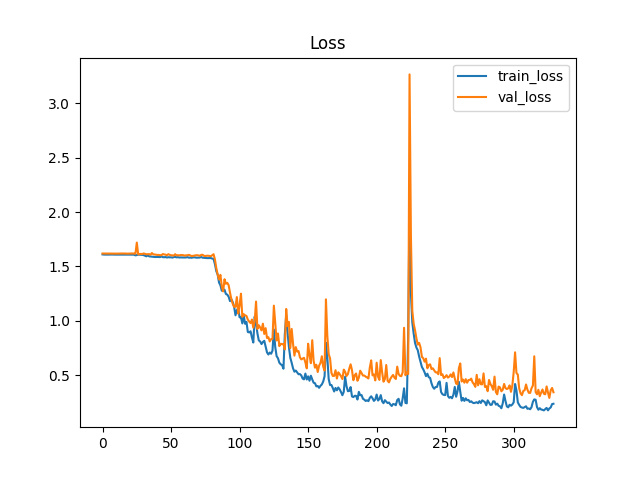
\includegraphics[height=10cm]{loss.png}
  \centering
  \caption{Wykres funkcji straty}
\end{figure}

Użyty optymalizator to $Adam$ ze współczynnikiem uczenia $0.001$
 Uzyskana precyzja to ok. 90\% (rys. 4). Wykorzystaliśmy wszystkie cechy (3 osie żyroskopu, 3 osie akcelerometru, 3 osie magnetometru). Macierz błędów widoczna na rys. 5.

 \begin{figure}[H]
  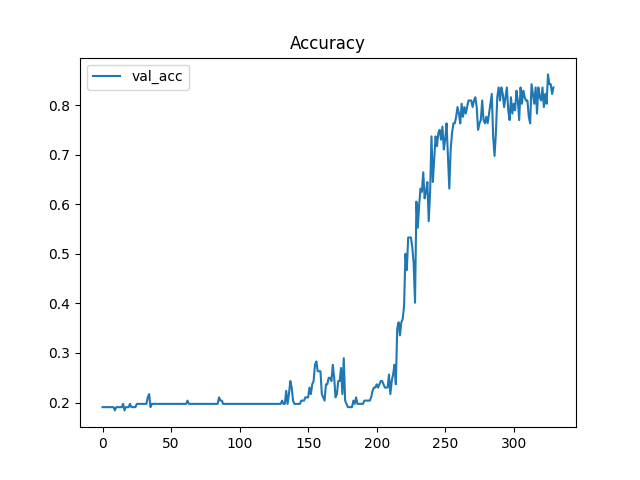
\includegraphics[height=9cm]{acc.png}
  \centering
  \caption{Wykres precyzji na zbiorze walidacyjnym}
\end{figure}

\begin{figure}[H]
  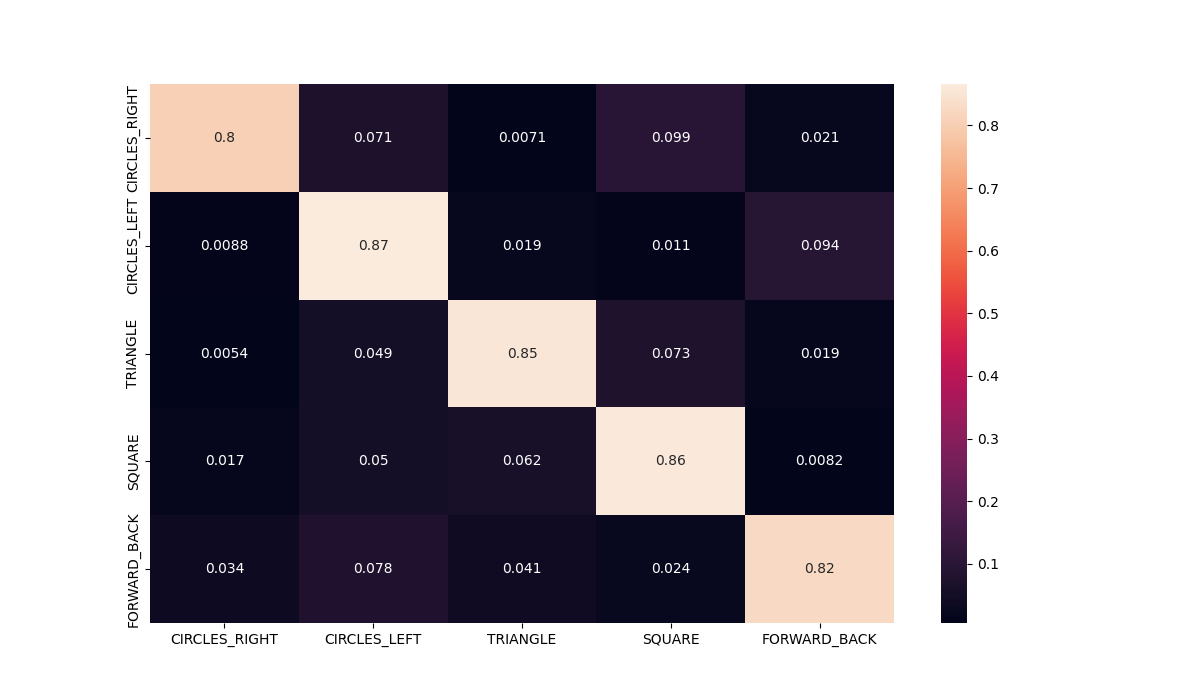
\includegraphics[height=9cm]{conf.png}
  \centering
  \caption{Wykres precyzji na zbiorze walidacyjnym}
\end{figure}

Co więcej, dostrzegliśmy różnice w zakresach odczytów używając kilku czujników IMU. Pomiary znacząco różniły się od siebie pomiędzy markami i modelami smartfonów. W związku z tym całe badanie oparliśmy na jednym urządzeniu Samsung Galaxy S10e.

\section{Inferencja}

Ze względu na to, że inferencja na smartfonie w przypadku rekurencyjnych sieci neuronowych jest trudna, zdecydowaliśmy się uruchomić zdalny serwer predykcji. Zastosowaliśmy iteracyjną metodologię prac nad projektem: 

\begin{enumerate}
  \item Wytrenuj model na lokalnym sprzęcie (laptop).
  \item Zbuduj obraz Dockera z wagami zawartymi w środku i wypchnij go do rejestru
  \item Na serwerze zdalnym: ściągnij obraz i uruchom serwer Flask
\end{enumerate}

Dzięki temu byliśmy w stanie szybko ewaluować jakość modelu. Aplikacja mobilna wykonuje żądanie HTTP POST do serwera inferencji, by ten zwrócił wyniki.

\section{Wnioski}

Na podstawie metryk modelu można stwierdzić, że decyzja o wykorzystaniu rekurencyjnej sieci neuronowej była trafna. Zaproponowana sieć neuronowa cechuje się wysoką skutecznością w zadaniu klasyfikacji ruchów z urządzenia IMU.

\section{Sprzęt}

Do pomiarów wykorzystaliśmy smartfon Samsung Galaxy S10e 2019 wyposażony w czujnik IMU. Implementację modelu wykonaliśmy we frameworku PyTorch. Trening sieci neuronowej była wykonywany na Apple Macbook M1 16GB.

\begin{thebibliography}{9}
  
  \bibitem{}
  Sepp Hochreiter and Jürgen Schmidhuber. 1997. Long short-term memory. Neural Comput. 9, 8 (1997), 1735–1780.

  \bibitem{}
  Rivera, Patricio, et al. "Recognition of human hand activities based on a single wrist imu using recurrent neural networks." Int. J. Pharma Med. Biol. Sci 6.4 (2017): 114-118.
  
  \bibitem{}
  Ashry, Sara, Reda Elbasiony, and Walid Gomaa. "An LSTM-based descriptor for human activities recognition using IMU sensors." Proceedings of the 15th International Conference on Informatics in Control, Automation and Robotics, ICINCO. Vol. 1. 2018.

  \bibitem{}
  Staudemeyer, Ralf C., and Eric Rothstein Morris. "Understanding LSTM--a tutorial into long short-term memory recurrent neural networks." (2019).
\end{thebibliography}

\end{document}